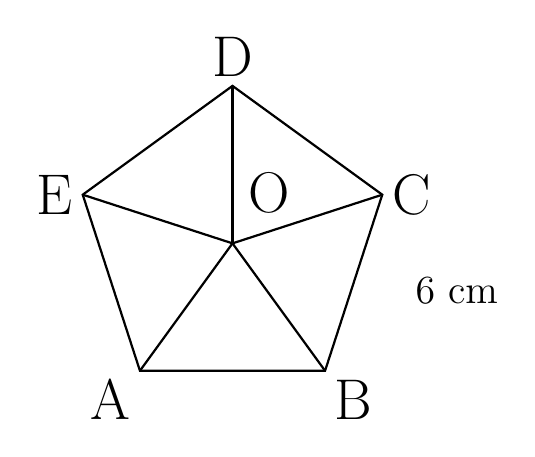
\begin{tikzpicture}[scale=1] % Reduced scale to make it smaller

    % --- Coordinates (Regular Pentagon) ---
    % Origin point where lines meet
    \coordinate (Origin) at (0,0);
    
    % Vertices set for a compact size
    \coordinate (D) at (90:2);   
    \coordinate (C) at (18:2);   
    \coordinate (B) at (306:2);  
    \coordinate (A) at (234:2);  
    \coordinate (E) at (162:2);  

    % --- Drawing ---
    % Drawing the outer perimeter ABCDE
    \draw[thick] (A) -- (B) -- (C) -- (D) -- (E) -- cycle;
    
    % Drawing lines from the center to each vertex
    \draw[thick] (Origin) -- (A);
    \draw[thick] (Origin) -- (B);
    \draw[thick] (Origin) -- (C);
    \draw[thick] (Origin) -- (D);
    \draw[thick] (Origin) -- (E);

    % --- Labels (Bigger Letters) ---
    % Using \huge to ensure the letters are large relative to the triangle
    \node[below left, font=\huge] at (A) {A};
    \node[below right, font=\huge] at (B) {B};
    \node[right, font=\huge] at (C) {C};
    \node[above, font=\huge] at (D) {D};
    \node[left, font=\huge] at (E) {E};
    
    % Placing O in the whitespace between lines (54 degrees)
    \node[font=\huge] at (54:0.8) {O};
    
    % Measurement label changed to "6 cm"
    \node[right, font=\Large] at (2.2, -0.6) {6 cm};

\end{tikzpicture}